\documentclass[a4paper,11pt]{report}
\usepackage{chuan_math_gkt}
\usetikzlibrary{angles,quotes,intersections,patterns,decorations.pathreplacing}
\chuanexamsetup

\begin{document}
\examfontsize

\examsecret{绝密$\bigstar$启用前}

\examtitle{2021年普通高等学校招生全国统一考试（全国甲卷理科）}{数\quad 学}

\examsection{一、选择题：本题共12小题，每小题5分，共60分. 在每小题给出的四个选项中，只有一项是符合题目要求的.}
\begin{examquestions}

\item 设集合 $M=\{x\mid 0<x<4\}$，$N=\{x\mid \dfrac13\leq x\leq5\}$，则 $M\cap N=$
\twochoices
{{$\left\{x\mid 0<x\leq\dfrac13\right\}$}}
{{$\left\{x\mid \dfrac13\leq x<4\right\}$}}
{$\{x\mid 4\leq x<5\}$}
{$\{x\mid 0<x\leq5\}$}

\item 为了解某地农村经济情况，对该地农户家庭年收入进行抽样调查，将农户家庭年收入调查数据整理得到如下频率分布直方图：

\begin{tightcenter}
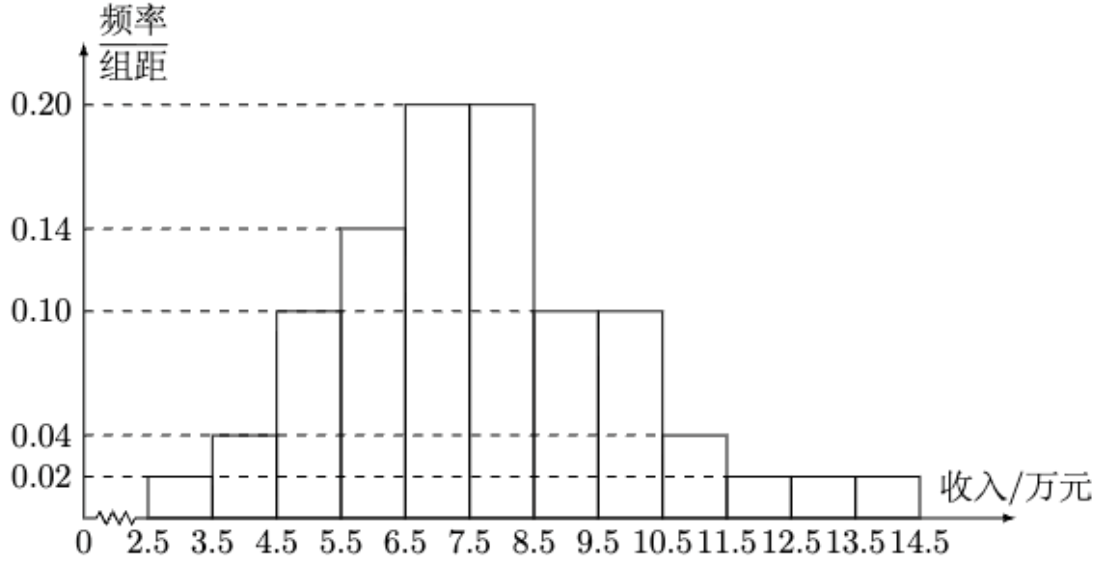
\includegraphics[width=8cm]{figures/2021_jia_li_image8.png}
\end{tightcenter}

根据此频率分布直方图，下面结论中不正确的是
\onechoices
{该地农户家庭年收入低于 $4.5$ 万元的农户比率估计为 $6\%$}
{该地农户家庭年收入不低于 $10.5$ 万元农户比率估计为 $10\%$}
{估计该地农户家庭年收入的平均值不超过 $6.5$ 万元}
{估计该地有一半以上的农户，其家庭年收入介于 $4.5$ 万元至 $8.5$ 万元之间}

\item 已知 $(1-\mathrm{i})^2z=3+2\mathrm{i}$，则 $z=$
\fourchoices
{\tallchoice{$-1-\dfrac32\mathrm{i}$}}
{\tallchoice{$-1+\dfrac32\mathrm{i}$}}
{\tallchoice{$-\dfrac32+\mathrm{i}$}}
{\tallchoice{$-\dfrac32-\mathrm{i}$}}

\item 青少年视力是社会普遍关注的问题，视力情况可借助视力表测量. 通常用五分记录法和小数记录法记录视力数据，五分记录法的数据 $L$ 和小数记录表的数据 $V$ 满足 $L=5+\lg V$. 已知某同学视力的五分记录法的数据为 $4.9$，则其视力的小数记录法的数据为（$\sqrt[10]{10}\approx1.259$）
\fourchoices{$1.5$}{$1.2$}{$0.8$}{$0.6$}

\item 已知 $F_1,F_2$ 是双曲线 $C$ 的两个焦点，$P$ 为 $C$ 上一点，且 $\angle F_1PF_2=60^\circ$，$|PF_1|=3|PF_2|$，则 $C$ 的离心率为
\fourchoices
{\tallchoice{$\dfrac{\sqrt7}{2}$}}
{\tallchoice{$\dfrac{\sqrt{13}}{2}$}}
{$\sqrt7$}
{$\sqrt{13}$}

\begin{minipage}[t]{0.82\linewidth}
\item 在一个正方体中，过顶点 $A$ 的三条棱的中点分别为 $E,F,G$. 该正方体截去三棱锥 $A-EFG$ 后，所得多面体的三视图中，正视图如图所示，则相应的侧视图是
\end{minipage}\hfill
\begin{minipage}[t]{0.13\linewidth}
\vspace{-1em}\centering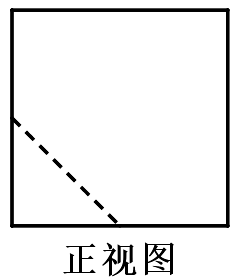
\includegraphics[width=\linewidth]{figures/2021_jia_li_image25.png}
\end{minipage}

\graphchoicesoneline
{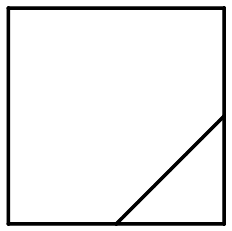
\includegraphics[width=1.4cm]{figures/2021_jia_li_image26.png}}
{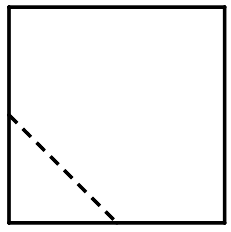
\includegraphics[width=1.4cm]{figures/2021_jia_li_image27.png}}
{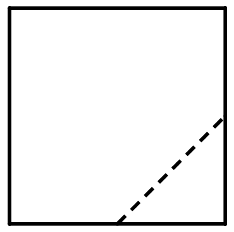
\includegraphics[width=1.4cm]{figures/2021_jia_li_image28.png}}
{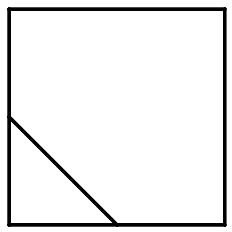
\includegraphics[width=1.4cm]{figures/2021_jia_li_image29.png}}

\item 等比数列 $\{a_n\}$ 的公比为 $q$，前 $n$ 项和为 $S_n$，设甲：$q>0$，乙：$\{S_n\}$ 是递增数列，则
\onechoices{甲是乙的充分条件但不是必要条件}{甲是乙的必要条件但不是充分条件}{甲是乙的充要条件}{甲既不是乙的充分条件也不是乙的必要条件}

\item $2020$ 年 $12$ 月 $8$ 日，中国和尼泊尔联合公布珠穆朗玛峰最新高程为 $8848.86$（单位：m），三角高程测量法是珠峰高程测量方法之一. 如图是三角高程测量法的示意图.

\begin{minipage}[t]{0.76\linewidth}
现有 $A,B,C$ 三点，且 $A,B,C$ 在同一水平面上的投影 $A',B',C'$ 满足 $\angle A'C'B'=45^\circ$，$\angle A'B'C'=60^\circ$. 由 $C$ 点测得 $B$ 点的仰角为 $15^\circ$，$BB'$ 与 $CC'$ 的差为 $100$；由 $B$ 点测得 $A$ 点的仰角为 $45^\circ$，则 $A,C$ 两点到水平面 $A'B'C'$ 的高度差 $AA'-CC'$ 约为（$\sqrt3\approx1.732$）
\end{minipage}\hfill
\begin{minipage}[t]{0.22\linewidth}
\vspace{-1.4em}\centering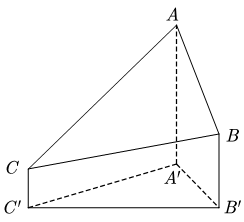
\includegraphics[width=\linewidth]{figures/2021_jia_li_image44.png}
\end{minipage}
\vspace{-0.5em}
\fourchoices{$346$}{$373$}{$446$}{$473$}

\vspace{-0.3em}

\item 若 $\alpha\in\left(0,\dfrac{\pi}{2}\right)$，$\tan2\alpha=\dfrac{\cos\alpha}{2-\sin\alpha}$，则 $\tan\alpha=$
\fourchoices
{\tallchoice{$\dfrac{\sqrt{15}}{15}$}}
{\tallchoice{$\dfrac{\sqrt5}{5}$}}
{\tallchoice{$\dfrac{\sqrt5}{3}$}}
{\tallchoice{$\dfrac{\sqrt{15}}{3}$}}

\vspace{-0.5em}
\item 将 $4$ 个 $1$ 和 $2$ 个 $0$ 随机排成一行，则 $2$ 个 $0$ 不相邻的概率为
\fourchoices
{\tallchoice{$\dfrac13$}}
{\tallchoice{$\dfrac25$}}
{\tallchoice{$\dfrac23$}}
{\tallchoice{$\dfrac45$}}

\item 已知 $A,B,C$ 是半径为 $1$ 的球 $O$ 的球面上的三个点，且 $AC\perp BC$，$AC=BC=1$，则三棱锥 $O-ABC$ 的体积为
\fourchoices
{\tallchoice{$\dfrac{\sqrt2}{12}$}}
{\tallchoice{$\dfrac{\sqrt3}{12}$}}
{\tallchoice{$\dfrac{\sqrt2}{4}$}}
{\tallchoice{$\dfrac{\sqrt3}{4}$}}

\vspace{-0.5em}
\item 设函数 $f(x)$ 的定义域为 $\mathbb R$，$f(x+1)$ 为奇函数，$f(x+2)$ 为偶函数，当 $x\in[1,2]$ 时，$f(x)=ax^2+b$. 若 $f(0)+f(3)=6$，则 $f\left(\dfrac92\right)=$
\fourchoices
{\tallchoice{$-\dfrac94$}}
{\tallchoice{$-\dfrac32$}}
{\tallchoice{$\dfrac74$}}
{\tallchoice{$\dfrac52$}}

\end{examquestions}

\examsection{二、填空题：本题共4小题，每小题5分，共20分.}
\begin{examquestions}[start=13]

\item 曲线 $y=\dfrac{2x-1}{x+2}$ 在点 $(-1,-3)$ 处的切线方程为 \blank.

\item 已知向量 $\vec a=(3,1)$，$\vec b=(1,0)$，$\vec c=\vec a+k\vec b$. 若 $\vec a\perp\vec c$，则 $k=$ \blank.

\item 已知 $F_1,F_2$ 为椭圆 $C:\dfrac{x^2}{16}+\dfrac{y^2}{4}=1$ 的两个焦点，$P,Q$ 为 $C$ 上关于坐标原点对称的两点，且 $|PQ|=|F_1F_2|$，则四边形 $PF_1QF_2$ 的面积为 \blank.

\begin{minipage}[t]{0.65\linewidth}
\item 已知函数 $f(x)=2\cos(\omega x+\varphi)$ 的部分图像如图所示，则满足条件 $\left(f(x)-f\left(-\dfrac{7\pi}{4}\right)\right)\left(f(x)-f\left(\dfrac{4\pi}{3}\right)\right)>0$ 的最小正整数 $x$ 为 \blank.
\end{minipage}\hfill
\begin{minipage}[t]{0.3\linewidth}
\vspace{-1em}\centering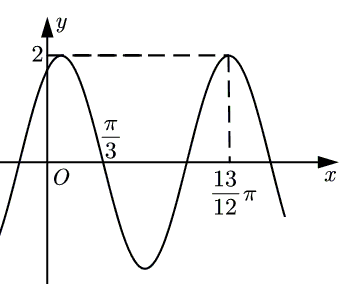
\includegraphics[width=\linewidth]{figures/2021_jia_li_image82.png}
\end{minipage}

\end{examquestions}

\examsection{三、解答题：共70分. 解答应写出文字说明、证明过程或演算步骤. 第17题～第21题为必考题，每个试题考生都必须作答. 第22、23题为选考题，考生根据要求作答.}
\begin{examanswers}[start=17]

\item（12分）

甲、乙两台机床生产同种产品，产品按质量分为一级品和二级品，为了比较两台机床产品的质量，分别用两台机床各生产了 $200$ 件产品，产品的质量情况统计如下表：

\begin{tightcenter}
{\renewcommand{\arraystretch}{0.9}
\begin{tabular}{|c|c|c|c|}
\hline
& 一级品 & 二级品 & 合计 \\ \hline
甲机床 & $150$ & $50$ & $200$ \\ \hline
乙机床 & $120$ & $80$ & $200$ \\ \hline
合计 & $270$ & $130$ & $400$ \\ \hline
\end{tabular}}
\end{tightcenter}

\subq{（1）}{甲机床、乙机床生产的产品中一级品的频率分别是多少？}

\subq{（2）}{能否有 $99\%$ 的把握认为甲机床的产品质量与乙机床的产品质量有差异？
附：$K^2=\dfrac{n(ad-bc)^2}{(a+b)(c+d)(a+c)(b+d)}$

\begin{tightcenter}
    {\renewcommand{\arraystretch}{0.9}
\begin{tabular}{|c|c|c|c|}
\hline
$P(K^2\geq k)$ & $0.050$ & $0.010$ & $0.001$ \\ \hline
$k$ & $3.841$ & $6.635$ & $10.828$ \\ \hline
\end{tabular}}
\end{tightcenter}
}

\item（12分）

已知数列 $\{a_n\}$ 的各项均为正数，记 $S_n$ 为 $\{a_n\}$ 的前 $n$ 项和，从下面 \gktcircled{1}\gktcircled{2}\gktcircled{3} 中选取两个作为条件，证明另外一个成立.

\gktcircled{1} 数列 $\{a_n\}$ 是等差数列；\gktcircled{2} 数列 $\{\sqrt{S_n}\}$ 是等差数列；\gktcircled{3} $a_2=3a_1$.

注：若选择不同的组合分别解答，则按第一个解答计分.

\item （19分）

已知直三棱柱 $ABC-A_1B_1C_1$ 中，侧面 $AA_1B_1B$ 为正方形，$AB=BC=2$，$E,F$ 分别为 $AC$ 和 $CC_1$ 中点，$D$ 为棱 $A_1B_1$ 上的点. $BF\perp A_1B_1$.

\noindent\begin{minipage}[t]{0.65\linewidth}
\subq{（1）}{证明：$BF\perp DE$；}

\subq{（2）}{当 $B_1D$ 为何值时，面 $BB_1C_1C$ 与面 $DFE$ 所成的二面角的正弦值最小？}

\end{minipage}\hfill
\begin{minipage}[t]{0.23\linewidth}
\vspace{-2.2em}\centering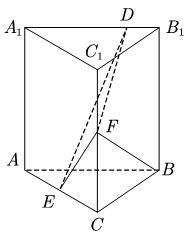
\includegraphics[width=\linewidth]{figures/2021_jia_li_image94.png}
\end{minipage}

\vspace{-3em}

\item（12分）

抛物线 $C$ 的顶点为坐标原点 $O$. 焦点在 $x$ 轴上，直线 $l:x=1$ 交 $C$ 于 $P,Q$ 两点，且 $OP\perp OQ$. 已知点 $M(2,0)$，且 $\odot M$ 与 $l$ 相切.

\subq{（1）}{求 $C$，$\odot M$ 的方程；}

\subq{（2）}{设 $A_1,A_2,A_3$ 是 $C$ 上的三个点，直线 $A_1A_2$，$A_1A_3$ 均与 $\odot M$ 相切. 判断直线 $A_2A_3$ 与 $\odot M$ 的位置关系，并说明理由.}

\item（12分）

已知 $a>0$ 且 $a\ne1$，函数 $f(x)=\dfrac{x^a}{a^x}(x>0)$.

\subq{（1）}{当 $a=2$ 时，求 $f(x)$ 的单调区间；}

\subq{（2）}{若曲线 $y=f(x)$ 与直线 $y=1$ 有且仅有两个交点，求 $a$ 的取值范围.}

\item（10分）【选修4-4：坐标系与参数方程】

在直角坐标系 $xOy$ 中，以坐标原点为极点，$x$ 轴正半轴为极轴建立极坐标系，曲线 $C$ 的极坐标方程为 $\rho=2\sqrt2\cos\theta$.

\subq{（1）}{将 $C$ 的极坐标方程化为直角坐标方程；}

\subq{（2）}{设点 $A$ 直角坐标为 $(1,0)$，$M$ 为 $C$ 上的动点，点 $P$ 满足 $\vec{AP}=\sqrt2\vec{AM}$，写出 $P$ 的轨迹 $C_1$ 的参数方程，并判断 $C$ 与 $C_1$ 是否有公共点.}

\vspace{1em}
\noindent\begin{minipage}[t]{0.65\linewidth}
\item（10分）【选修4-5：不等式选讲】

已知函数 $f(x)=|x-2|$，$g(x)=|2x+3|-|2x-1|$.

\subq{（1）}{画出 $y=f(x)$ 和 $y=g(x)$ 的图像；}

\subq{（2）}{若 $f(x+a)\geq g(x)$，求 $a$ 的取值范围.}
\end{minipage}\hfill
\begin{minipage}[t]{0.3\linewidth}
\vspace{0em}\centering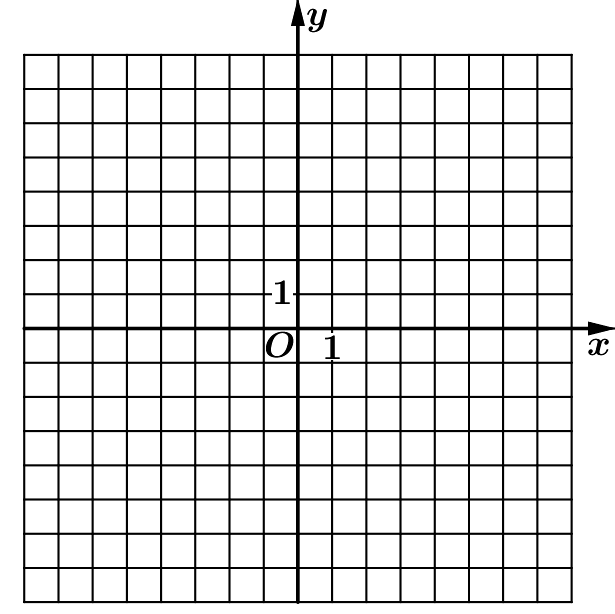
\includegraphics[width=\linewidth]{figures/2021_jia_li_image119.png}
\end{minipage}

\end{examanswers}

\end{document}